\documentclass[graphics]{beamer}

\usepackage{graphicx}
\usepackage{verbatim}
\usepackage{wrapfig}
\useoutertheme{shadow}
%\usecolortheme{orchid}
\usecolortheme{seahorse}


% math commands
\newcommand{\be}{\begin{eqnarray}}
\newcommand{\ee}{\end{eqnarray}}
\newcommand{\beq}{\begin{equation}}
\newcommand{\eeq}{\end{equation}}
\def\simless{\mathbin{\lower 3pt\hbox
      {$\rlap{\raise 5pt\hbox{$\char'074$}}\mathchar"7218$}}}
\def\simgreat{\mathbin{\lower 3pt\hbox
      {$\rlap{\raise 5pt\hbox{$\char'076$}}\mathchar"7218$}}} %> or of order

% variables

\def\toonscale{0.45}
\def\mboxy#1{\mbox{\small #1}}


\begin{comment}
\AtBeginSection[]{
  \frame{
    \frametitle{Outline}
    \tableofcontents[currentsection]
  }
}
\end{comment}

\title{The universe probed by coherent radiation: gravitational waves and FRBs
}
%\subtitle{interim update}
\author[U. Pen]{Ue-Li Pen
\\ Dylan Jow, Job Feldbrugge, Neil Turok, Emily Tyhurst, Fangxi Lin 
}
\date{August 12, 2021}


\begin{document}

%\section*{Introduction}
\section{Lenses}

\begin{comment}
  \subsection{Outline}

  \frame{
    \frametitle{Outline}
    \tableofcontents
  }
\end{comment}

\frame{\maketitle}



  \frame{
    \frametitle{Lenses}
    \begin{itemize}
        \item Coherent sources: forms interference pattern
        \item expected (observed) for FRBs, GWs
        \item wave effects: Eikonal vs Picard-Lefschetz
        \item Gravitational Lensing: micro, macro
        \item Plasma lensing
    \end{itemize}
  }

  \frame{
\vspace{-0.5in}
    \frametitle{Coherence}
    \begin{itemize}
    \item almost all astronomical (and terrestial) objects are {\it resolved} under
      multipath propagation and do not scintillate diffractively
    \item  unresolved {\it coherent} sources exhibit interference
      pattern through multipath propagation
    \item only pulsars and FRBs are known to fully modulate on
      diffractive time scales
    \item observed FRB plasma lensing implies gravitational (micro-)lensing
    \end{itemize}
  }


  \frame{
\vspace{-0.25in}
    \frametitle{Initial results}
    \begin{itemize}
        \item FRB110523: galactic scintillation of scattering tail
          shows that scattering occuring in host, not along the path  (Masui+2015)
        \item FRB201124A: measurement of scintillation time
          scale/frequency (Main+2021)
        \item black widow PSR: direct resolution of emission region
          (Main+2018, Nature, 557, 522)
        \item local screen resolving of crab GP: Main+2021, ApJ 915, 65
        \item crab: evidence for high Lorentz factor $\gamma \sim
          10^4$ with small $\Delta \gamma/\gamma < 0.01$  (Bij+2105.08851)
        \item empirical support for $\gamma^2$ free electron laser
          (Lyutikov++2021), moving mirror (Colgate+1971)
        \item promising tool for FRBs
    \end{itemize}

  }


  \frame{
\vspace{-0.5in}
    \frametitle{New Observables}
    \begin{itemize}
    \item microlensing: instant time delay: stars, planets (Jow+20,Kadar+21)
    \item weak lensing: imaginary image allows time delay measurement (Jow+21)
    \item macrolensing: potentially nano-second delay -- universe
      expands! (Wucknitz+21)
    \item dimensionless strain picoseconds/Giga years $h\sim \Delta t/t \sim 10^{-26}$:
      competitive with LIGO, LISA, etc (Yang+2017)
    \end{itemize}
\vspace{-0.4in}
\begin{center}
\includegraphics[width=4.1in]{Figures/lensing-VLBI.png}
\end{center}
\vspace{-0.6in}
  }


  \frame{
\vspace{-0.5in}
    \frametitle{Wave Optics History}
    \begin{itemize}
    \item Fermat, Huygens, Feynmann
    \item Picard-Lefschetz (19th century), Witten (2010)          
    \item concept: Oscillatory Kirchoff path integral
    \item sum over all possible paths, weighted by phase
    \item new phenomena: imaginary images, diffraction
    \item Numerical challenges (e.g. Grillo and Cordes 2018)            
    \end{itemize}
  }


  \frame{
\vspace{-0.25in}
    \frametitle{Optics: Geometric, Eikonal, Wave, P-L}
    \begin{itemize}
        \item Consider 1-D lens
        \item lensing potential $\Psi(\theta)$
        \item deflection $\Psi'$
        \item simplify for $D_{\rm ds}=\infty$
    \end{itemize}
\vspace{-0.5in}\hspace{2.5in}\includegraphics[width=1.5in]{Figures/lens.png}

  }


  \frame{
\vspace{-0.25in}
    \frametitle{Huygen's Principle: Path Integral}
    \begin{itemize}
        \item $A=\int e^{i S(\theta,\mu)} d\theta$ 
        \item $S=\nu [(\theta-\mu)^2+\Psi(\theta)]$
        \item Highly oscillatory integral, even for $\Psi=0$
        \item Stationary phase points: $\partial_\theta S=0$ leads to (complex)
          Eikonal images $\theta_i$.
        \item flux/phase through curvature expansion (known as {\it
            steepest descent}): exact as $\nu \rightarrow \infty$
        \item Geometric limit considers only {\it Real} $\theta_i$ and
          absolute value of the action $S$, giving up phase
          information
        \item Geometric optics applicable at short wavelengths for
          extended sources
          (e.g. optical gravitational lensing of finite size sources,
          stars)          
    \end{itemize}
  }

  \frame{
\vspace{-0.5in}
    \frametitle{Imaginary Images}
    \begin{itemize}
    \item consider ``rational lens'' potential $\psi(\theta)=\alpha/(1+\theta^2)$
    \item Geometric/eikonal images at $\psi'=\theta$
    \item 5 roots.  1 or 3 real roots, rest imaginary
    \item P-L: at most one imaginary image contributes!
    \item imaginary image can be brighter than unlensed real image
    \item one imaginary image more real than the others
    \end{itemize}
  }


  \frame{
%\vspace{-0.5in}
    \frametitle{Rational 1-D lens}
\begin{center}
\includegraphics[width=3.1in]{Figures/theta-beta.eps}
\end{center}
  }

  \frame{
\vspace{-0.5in}
    \frametitle{Picard-Lefschetz Theory}
    \begin{itemize}
    \item descend integral along real line along Morse function Im(S)
    \item contour deforms into finite number of Thimbles of constant
      phase with maximum at saddle point (extrema $dS=0$)
    \item correctly identifies relevant saddle points
    \item resolves numerical challenges of oscillatory integral
    \item complex analysis works in multiple variables
    \item elevates concept of ``image'' deep into wave optics
    \item multiple public implementations (Feldbrugge+, Jow+)
    \end{itemize}
  }



  \frame{
\vspace{-0.5in}
    \frametitle{Picard-Lefschetz Theory}

\includegraphics[width=4.5in]{Figures/thimbles.png}

Feldbrugge+2019
  }


  \frame{
\vspace{-0.5in}
    \frametitle{New Observables}
    \begin{itemize}
    \item weak lensing: imaginary image allows time delay measurement (Jow+21)
    \item strong lensing: delay measurements enable measurement of
      co-linearity (Jow++21)
    \item microlensing: instant time delay, planets (Jow+20)
    \item macrolensing: potentially nano-second delay -- universe
      expands! (Wucknitz+21)
    \item dimensionless strain picoseconds/years $h\sim \Delta t/t \sim 10^{-20}$:
      competitive with LIGO, etc
    \end{itemize}
  }


  \frame{
%\vspace{-0.5in}
    \frametitle{A2 fold}
\begin{center}
\vspace{-0.3in}
\includegraphics[width=4.5in]{Figures/rational_fold_crossing.pdf}
\end{center}
  }


  \frame{
\vspace{-0.5in}
    \frametitle{Macrolensing}
    \begin{itemize}
    \item Wucknitz+ 2021
    \item alternate approach to cosmography
    \item triangulation: lens model+time delay measurement = $H_0$
    \item weak link has been lens model
    \item Wave optics: time delay observable to nanoseconds
    \item For repeating FRB, dominated by galaxy transverse
      motion. then cosmic expansion
    \item individual macrolens images split into microlens images by stars
    \end{itemize}
  }



  \frame{
\vspace{-0.5in}
    \frametitle{Discussion}
    \begin{itemize}
    \item Eikonal effects applicable to compact radio sources,
      e.g. FRBs, pulsars
    \item full wave
effect dominates for long wavelengths as Fresnel scale is bigger then Einstein radius
    \item down to planet size
    \item gravitational waves:  LIGO, LISA, PTA
    \item PTA sources generically in wave limit under strong and weak
      gravitational lensing.  Requires PSR distances, e.g. Boyle+2012
    \end{itemize}
  }





  \frame{
\vspace{-0.5in}
    \frametitle{Conclusions}
    \begin{itemize}
    \item wave optics changes nature of observables: one of the potentially most
      precise measurements in physics
    \item coherent radio waves (FRBs, pulsars): described by Eikonal
      away from caustics/catastrophies for objects more massive than planets
    \item long wavelength GW (LIGO, LISA, PTA): full wave effects, P-L theory
    \item importance of imaginary images, Stokes phenomena
    \end{itemize}
  }

\end{document}
